\cleartooddpage[\thispagestyle{empty}]
\chapter{Gamma Rays}

As this thesis attempts to discern the presence of dark matter from gamma rays, a discussion on gamma rays and their properties is necessary.
These discussions revolve around three main topics: astrophysical mechanisms for creating gamma rays, gamma-ray-induced air showers in the Earth's atmosphere, and the different features of the Galactic Center relevant to gamma rays and this thesis.


\section{Methods of Creation}

There are three astrophysical mechanisms that are predicted to produce gamma rays at TeV energies.
The leptonic mechanism is when gamma rays' last energetic interaction is with electrons, while the hadronic mechanism is when gamma rays are created via proton interactions.
The third mechanism, one explored in this thesis, is when two WIMP dark matter particles annihilate either directly or indirectly into gamma rays.

In leptonic production, stars and galaxies have their own magnetic fields, and also emit electrons.
Electrons passing through these magnetic fields emit synchrotron photons, which can then scatter off of other electrons, gaining more energy. (reword this??)
After multiple cycles of this, a small fraction of the original photon population can gain TeV energies.
Other mechanisms can increase the number of TeV photons produced by a source, including stronger magnetic fields, breaking/reconnecting magnetic fields, as well as nearby ambient clouds of electrons.

In hadronic processes, protons are first accelerated by fermi acceleraton, emitted as part of a jet, or other mechanisms.
Then, upon striking an ambient atom, the proton will decay into $\pi^{+}$, $\pi^{-}$, and $\pi^{0}$.
The $\pi^{0}$ then quickly (<1sec) decays into a $\gamma\gamma$ pair, with \nicetilde $\frac{1}{10}$th the original proton's energy.
Much of the diffuse gamma ray component of the galactic disk is believed to be due to extra-galactic high-energy protons colliding with the atoms of the dusty galactic plane.(cite??)


\subsection{Dark Matter Interactions}
As discussed in various extensions of SUSY(cite??), dark matter may present itself to be studied through several kinds of particle interactions, organizable in three general types.
Direct interactions: $\chi-s \rightarrow \chi-s$ (switch all of these to feynman diagrams!??) Collider interactions: $s-s \rightarrow \chi-\chi$, and Indirect detection: $\chi-\chi \rightarrow s-s$.
In Direct interactions, detection masses look for the movements of standard model particles, recoiling from a collision with a passing dark matter particle.
In Collider interactions, two standard model particles are accellerated into each other, and the resulting cascade of particles is analyzed for missing energy, hinting that a dark matter particle was created.
In Indirect detection, the subject of this thesis, the dark matter particles may annihilate out in deep space, producing pairs of standard model particles that eventually transform into gamma rays.

Primarily, the search detailed in this thesis looks for $\chi\chi \rightarrow q\overline{q} \rightarrow \gamma\gamma$.
Top and bottom quarks are considered


%Indirect Detection: dark-dark => sm-sm
%Direct Detection  : dark-sm => dark-sm
%Collider Detection: sm-sm => dark-dark

%Indirect can produce gamma rays via quark/lepton annihilation (??)
%dark-dark => t-t => gamma-gamma
%dark-dark => b-b => gamma-gamma


\section{Atmospheric Shower}
(this entire section needs more citations!??)

When a gamma ray, proton, or other particle strikes an atom of Earth's atmosphere, it can set off a cascade of energetic particles called an air shower.
When the primary particle is a gamma ray, an electron, or a positron, it creates an electromagnetic shower.
When the primary is a proton or other baryon, it creates a hadronic shower.
During either cascade of particles, any charged particles travelling at $v_{particle} > c_{atmosphere}$ will create Cherenkov photons, UV- and Visible-spectrum photons that are then imaged and recorded by the VERITAS observatory.

(image of particle cascade diagram??)

Electromagnetic air showers are started by a high energy (\nicetilde TeV) electron or gamma-ray, and produce a cascade of electrons, positrons, and photons, where initially each successive generation of particles tends to have more particles and less energy per particle than the last.
The primary gamma ray will interact with an atmospheric atom, producing a $e^{-}e^{+}$ pair, each with roughly half the primary gamma ray's energy.
The $e^{-}$ and $e^{+}$ will emit some photons through bremstrahlung radiation, until they only have a few MeV of kinetic energy, after which other energy loss mechanisms (compton, etc) dominate.
The photons created during the shower go on to produce more $e^{-}e^{+}$ pairs, though as each newly created particle has less energy than its parent particle, eventually the photons in the shower don't have enough energy to produce additional $e^{-}e^{+}$ pairs, and the shower dies off.

As most (\nicetilde 99\%??) of detected air showers are due to protons and not gamma rays, understanding the differences between hadronic showers and electromagnetic showers becomes useful in removing unwanted proton air showers and preserving gamma-ray air showers within the reconstruction software, sometimes referred to as gamma-hadron separation.
Hadronic showers start with a primary \nicetilde TeV proton that interacts with an atmospheric atom.
This proton then converts into a $\pi^{+}\pi^{-}\pi^{0}$, each with roughly \nicetilde 33\% (it varies though??) of the initial proton's energy.
The $\pi^{+}$ and $\pi^{-}$ can travel far from the main axis of the primary particle, then produce $\mu\nu$ pairs.
The $\pi^{0}$ quickly decays into $\gamma\gamma$, which then each start their own electromagnetic shower.
The $\pi^{+}$ and $\pi^{-}$ can have a large transverse momentum (relative to the primary shower axis), and also have longer decay time (??), both of which contribute to creating sub-cascades of showers further away from the primary particle axis, which tends to cause hadronic showers (and their resulting Cherenkov images) to be wider than a purely electromagnetic shower of the same length. 

\begin{figure}[ht]
  \begin{center}
    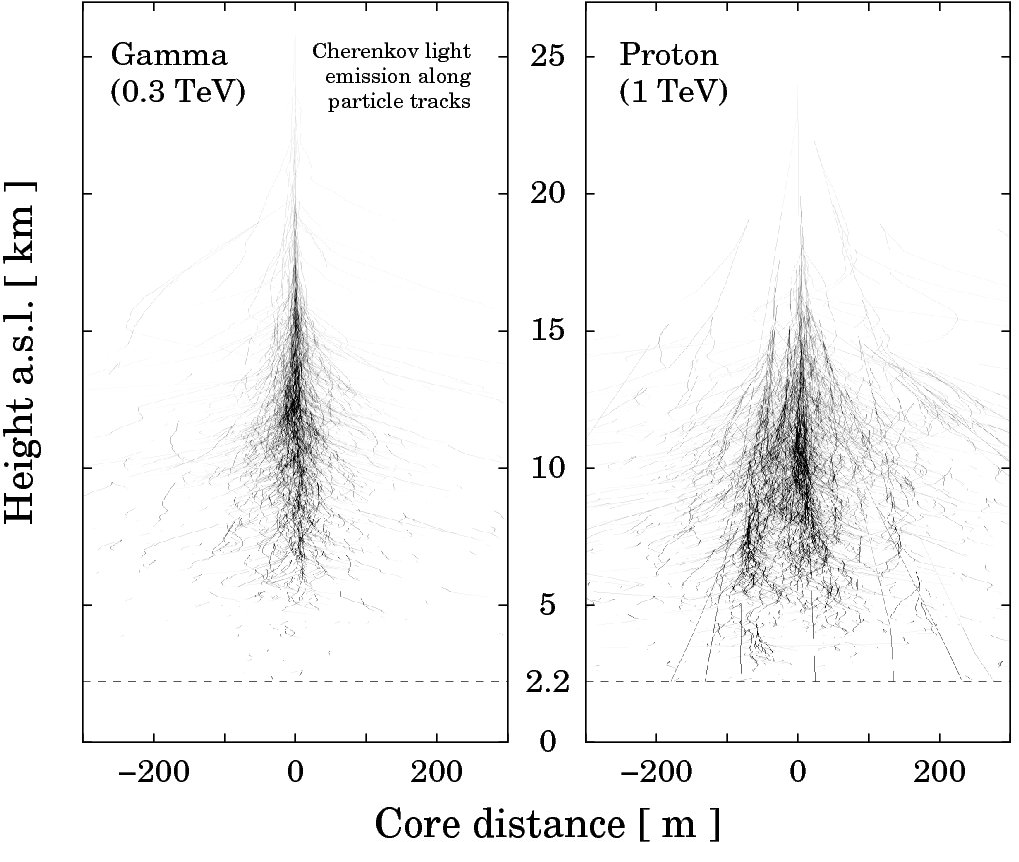
\includegraphics[width=0.95\textwidth]{images/showers_gamma_proton}
    \caption[Gamma Ray and Proton Showers]{A gamma ray shower alongside a proton shower.\cite{Bernlohr2008149}}\label{fig:gamma_vs_proton_airshower}
  \end{center}
\end{figure}

(image of proton vs gamma shower cherenkov image??)


\section{Galactic Center}
The galactic center is a complex region of space, with many astrophysical sources of gamma rays.
A disk of dust lies along the galactic plane, acting as an interaction medium for diffuse proton cosmic rays.
Nearby supernova remnants also produce gamma-rays as their expanding shell interacts with ambient dust.
The immediate area surrounding the galactic center a point-source emitter of gamma rays, though this mechanism is uncertain.

% black hole
Through kinematic observations of nearby stars, the galactic center is suspected to have a black hole, on the order of $10^6 M_{\odot}$. ??
The Galactic Center also is a source of TeV gamma rays, though the mechanism that produces them is still under debate.
% http://adsabs.harvard.edu/cgi-bin/bib_query?arXiv:1511.01159
One possibility is that the supermassive black hole emits particles, which convert into TeV gamma rays, while the second possibility suggests a nearby Pulsar Wind Nebula may be providing the gamma-ray-parent particles.
While the Galactic Center emits gamma rays, this emission is point-like to ground-based gamma ray telescopes. (rewrite this!??)
This analysis instead focuses on the gamma ray flux outside this point-like inner angular region. (citation!??)

The disk of gas present in the galactic plane acts as an interaction medium for passing cosmic rays, both from nearby galactic accelerators and from extragalactic sources.
These high-energy protons collide with the dust, shattering into $\pi^{\pm,0}$.
The $\pi^0$ then decays into two gamma rays ??, providing the diffuse emission.
The spectrum of this emission is ??.


